% !TeX spellcheck = en_US
\chapter{Sim-to-Real Measures in the Arm Controller}\label{ch:app-controller}%
\sloppy%

The student commands the arm through the operational-space impedance law of \eqref{eq:osc}, and the same law runs in training and on the physical \ac{FR3} (Section~\ref{sec:action-contract}). The two arms behind that law differ. The training arm is a gravity-free PhysX articulation, whereas the physical arm has gearbox friction that depends on joint velocity and posture. This chapter documents what was added to the deployment controller to narrow that gap, and the measurements behind each addition. It also covers \emph{ros-sim}, a MuJoCo simulation of the workcell that runs the same ROS~2 stack and the same C++ controller as the physical robot and is used to rehearse every hardware rollout.

Each section separates two kinds of statement. \emph{Results} are read from logged data. \emph{Interpretation} explains the results and is marked as such. Every result states the condition it was measured under. Wrenches are given in N and N\,m, pose errors in mm and degrees, and joint quantities in rad and rad/s. ``Dead zone'' always means the task-wrench dead zone defined in Section~\ref{sec:app-ctrl-dz-train}.

Table~\ref{tab:ctrl-fixed} lists the controller settings that all measurements in this chapter share.

\begin{table}[htb]%
    \centering%
    \caption[Settings of the deployment Cartesian impedance controller]{Settings of the deployment Cartesian impedance controller shared by all measurements in this chapter. Hardware runs without friction compensation differ only in that term. ros-sim differs in the model source (built-in kinematic model instead of libfranka), in gravity (off in the scene instead of compensated), in friction compensation (off by default), and in the dead zone, which can only be set there.}%
    \label{tab:ctrl-fixed}%
    \resizebox{\textwidth}{!}{%
    \begin{tabular}{ll}
        \toprule
        Quantity & Value \\
        \midrule
        translational / rotational stiffness $\mat{K}_p$ & 565\,N/m / 28\,N\,m/rad \\
        damping $\mat{K}_d$ & $2\sqrt{\mat{K}_p}$, i.e.\ 47.5\,N\,s/m / 10.6\,N\,m\,s/rad \\
        nullspace & stiffness 10, mass-weighted dynamically consistent projector \\
        Coriolis compensation & off, as in training \\
        policy clip (per axis, 1\,kHz, on the policy goal) & 0.02\,m / 0.097\,rad \\
        tracking-fault limits (policy phase) & 0.08\,m / 0.35\,rad \\
        transition-clip ceilings / fault ceilings & 0.05\,m / 0.25\,rad, 0.1\,m / 0.5\,rad \\
        tool offset in the flange frame & $(-0.058208, -0.028713, 0.173779)$\,m \\
        joint torque limits & 87\,N\,m (j1--j4), 12\,N\,m (j5--j7) \\
        friction compensation $c_j$ / $v_s$ / $\tau_s$ & 0.3\,N\,m on every joint / 0.05\,rad/s / 0.3\,N\,m \\
        task-wrench dead zone & 0 on hardware, selectable in ros-sim \\
        \bottomrule
    \end{tabular}}
\end{table}%

\section{Task-Wrench Dead Zone in Training}\label{sec:app-ctrl-dz-train}

\paragraph{Purpose and implementation.} The teacher is trained with a dead zone on the task wrench, which models the unreliability of the controller at low forces. Let $\vec{w}=\mat{K}_p\vec{e}-\mat{K}_d\dot{\vec{x}}$ be the task wrench of \eqref{eq:osc} in the robot base frame and $\vec{d}\in\R^6_{\ge0}$ the thresholds. Each component is shrunk toward zero,
\begin{equation}\label{eq:dead-zone}
  \tilde{w}_i=\begin{cases}0, & |w_i|<d_i,\\ \operatorname{sign}(w_i)\,(|w_i|-d_i), & \text{otherwise,}\end{cases}\qquad i=1,\dots,6,
\end{equation}
and $\tilde{\vec{w}}$ replaces $\vec{w}$ in $\mat{J}^{\mathrm{T}}\vec{w}$. The nullspace term is not affected. The thresholds are drawn as $\vec{d}\sim U(\vec{0},\vec{d}_{\max})$ with $\vec{d}_{\max}=[5,5,5\,\mathrm{N},1,1,1\,\mathrm{N\,m}]$ at every reset and again every 2\,s, when they are redrawn for all environments at once. The training arm has gravity disabled. Recipes with physics randomization also add joint friction, scaling a nominal 0.2\,N\,m per joint by a factor from $U(0.8,2.0)$.

At the gains of Table~\ref{tab:ctrl-fixed}, the worst-case thresholds correspond to a band of $5/565=8.8$\,mm in position and $1/28\,\mathrm{rad}=2.0\degree$ in orientation, inside which the spring produces no wrench. With zero position error, a pure damping wrench is also removed below $5/47.5=0.105$\,m/s and $1/10.6=0.094$\,rad/s.

\paragraph{Recipes.} Three dataset recipes treat the dead zone differently:
\begin{itemize}
  \item the \emph{extended-randomization} recipe inherits the teacher's dead zone together with gain noise ($\ell=0.41$), a random smoothing factor $U(0.025,0.1)$, the arm joint friction factor $U(0.8,2.0)$, and nut-depth randomization.
  \item the \emph{proprio-friction} recipe sets the dead zone to zero, fixes the gains and the smoothing factor at 0.0625, and keeps the joint friction factor $U(0.8,2.0)$.
  \item the \emph{return-dead-zone} student adds a dead zone only during release and return. It is drawn per return and per axis from zero to a configured maximum and set back to zero when the arm is handed back to the policy.
\end{itemize}

\paragraph{Interpretation.} The following reading is an analysis of \eqref{eq:dead-zone}, not a measurement. On a gravity-free arm, the dead zone is a hole in the stiffness: inside the band no task wrench acts, and the hand floats. In free space this resembles static friction, because a small error is not corrected. In contact the two differ. A frictionless arm inside the band offers no resistance, so contact forces between fingers and nut can move the hand and re-center the grasp. A physical arm resists the same contact forces through joint friction. The dead zone is also memoryless and independent of speed, whereas joint friction acts in joint space, depends on the posture through the Jacobian, and depends on the direction of motion. Sections~\ref{sec:app-ctrl-rollout} to~\ref{sec:app-ctrl-fit} test which of these properties matter for deployment.

\section{Controller Additions for Deployment}\label{sec:app-ctrl-additions}

The deployment controller is a ros2\_control plugin whose control law reproduces \eqref{eq:osc}. Two terms were added to it for deployment.

\paragraph{Dead zone in ros-sim.} The controller implements \eqref{eq:dead-zone} component-wise and applies it to the task wrench before $\vec{\tau}_{\mathrm{task}}=\mat{J}^{\mathrm{T}}\tilde{\vec{w}}$. The thresholds default to zero and can only be set in ros-sim, either to $\vec{d}_{\max}$ (the worst case) or to six explicit values. Training redraws the thresholds at every reset and every 2\,s, whereas ros-sim holds them fixed for a whole run, so the worst case is the upper end of the training distribution. Training expresses the wrench in a world frame that is the robot base rotated by $\pi$ about $z$. This flips the signs of $x$ and $y$ but not the magnitudes, so the base-frame dead zone gives the same result. Two unit tests check that the controller's dead zone matches the training implementation component-wise and that it is off by default.

\paragraph{Joint friction compensation on hardware.} Friction compensation adds a Coulomb torque per joint before the torque clamp and the rate limiter,
\begin{equation}\label{eq:friction-ff}
  \tau_{f,j}=c_j\left[s_j\operatorname{sign}(\dot{q}_j)+(1-s_j)\tanh\!\left(\frac{\tau_{\mathrm{imp},j}}{\tau_s}\right)\right],\qquad s_j=\min\!\left(1,\frac{|\dot{q}_j|}{v_s}\right),
\end{equation}
where $\vec{\tau}_{\mathrm{imp}}=\vec{\tau}_{\mathrm{task}}+\vec{\tau}_{\mathrm{null}}$ is the impedance torque, $c_j$ the Coulomb coefficient, $v_s$ the velocity scale, and $\tau_s$ the torque scale (Table~\ref{tab:ctrl-fixed}). While a joint moves faster than $v_s$, the compensation follows its velocity. Near standstill it follows the commanded impedance torque, so a joint that is asked to move receives the breakaway torque, and a joint at equilibrium ($\vec{\tau}_{\mathrm{imp}}\approx0$) receives none. The two blend linearly in $|\dot{q}_j|/v_s$. The coefficients are read only when the controller is configured, so switching friction compensation on or off requires a restart of the controller. Four unit tests cover the off state, the moving branch, the standstill branch, and the blend.

The value of 0.3\,N\,m was chosen from two earlier hardware runs, which are not among the runs analyzed in this chapter. According to the notes kept with the controller settings, the yaw clip in those runs asked the wrist joint for about 1\,N\,m, of which about 0.65\,N\,m was lost to joint friction (commanded $-1.0$\,N\,m, $-0.35$\,N\,m at the link). The wrist then turned at 22--28\degree/s instead of 37--41\degree/s, and the fingers reached the nut 0.3\,rad short of the simulated pre-rotation. The moving losses measured in those runs were 0.32--0.44\,N\,m on j2 and j5--j7, and 0.3\,N\,m was chosen to stay below all of them. The same notes report that 0.4\,N\,m per joint raised a student in ros-sim from 0 to 3 cycles in 450 steps.

\paragraph{Logged state.} Every controller cycle publishes a state message at 50\,Hz and, for recording, at 1\,kHz. It carries the goal, the clipped target, and the measured pose, the 6-D error, the wrench after the dead zone, $\vec{\tau}_{\mathrm{task}}$, $\vec{\tau}_{\mathrm{null}}$, the commanded torque, the filtered measured torque, the gravity torque, and the clip and fault limits in effect. In ros-sim, the wrench removed by the dead zone is therefore known exactly in every cycle as $\mat{K}_p\vec{e}-\mat{K}_d\dot{\vec{x}}-\tilde{\vec{w}}$.

\section{Rollouts in ros-sim with and without the Dead Zone}\label{sec:app-ctrl-rollout}

\paragraph{Purpose and method.} This comparison tests whether the training dead zone makes ros-sim reproduce the physical arm. The proprio-friction student $S_1$ was run three times in ros-sim without the dead zone and three times with the worst-case dead zone, without friction compensation and with the same runner settings as on hardware. It was compared with two hardware runs of the same student. One of them used friction compensation; for the other, the setting was not recorded. Every cycle is cut from its first policy sample and aligned on that step. For every observation channel, the RMS distance to the hardware mean is computed over the first 69 policy steps.

\paragraph{Results.} The hardware runs completed 3 and 6 cycles, which gives 9 hardware cycles. In ros-sim, five of six runs ended with a re-home failure (a 15\,s timeout of the controller manager), so the comparison has 3 cycles without the dead zone, none of them completed, and 4 cycles with the dead zone, one of them completed. Table~\ref{tab:ctrl-dz-rollout} summarizes the cycle metrics, Table~\ref{tab:ctrl-dz-distance} the observation distances, and Figure~\ref{fig:ctrl-dz-overlay} the traces.

\begin{table}[htb]%
    \centering%
    \caption[Per-cycle metrics with and without the dead zone in ros-sim]{Per-cycle metrics of the proprio-friction student $S_1$ on hardware and in ros-sim with and without the worst-case dead zone. Ranges are over cycles. The return error is taken at the last sample of the return, when the re-home gate of 30\,mm and $25\degree$ is met. Grip width is the median fingertip separation over the last 30 policy steps.}%
    \label{tab:ctrl-dz-rollout}%
    \resizebox{\textwidth}{!}{%
    \begin{tabular}{lccc}
        \toprule
        Metric & Hardware & ros-sim, worst-case dead zone & ros-sim, no dead zone \\
        \midrule
        cycles analyzed & 9 & 4 & 3 \\
        policy steps per cycle & 84--98 & 93--94 (112 in one cycle 2) & 69--70 \\
        return error at the gate & 11.5--12.9\,mm, 24.8--25.0\degree & 17.2--17.8\,mm, 24.5--25.0\degree & 3.2\,mm, 14.2--15.3\degree \\
        lowest grasp height & 108.8--113.3\,mm & 121.2--122.9\,mm & 114.3--114.7\,mm \\
        grip width & 31.7--35.2\,mm & 6.1--8.0\,mm (28.2 in one cycle) & 6.2\,mm \\
        peak j5 angle & 1.89--1.98\,rad & 2.05--2.20\,rad & 1.68--1.69\,rad \\
        \bottomrule
    \end{tabular}}
\end{table}%

\begin{table}[htb]%
    \centering%
    \caption[Observation distances to the hardware mean]{RMS distance of observation groups to the hardware mean over the first 69 policy steps of every cycle. ``Hardware spread'' is the distance of the hardware cycles to their own mean. Joint positions in rad, velocities in rad/s, previous actions in normalized units, pad forces divided by 20\,N, torques divided by the joint limit.}%
    \label{tab:ctrl-dz-distance}%
    \resizebox{\textwidth}{!}{%
    \begin{tabular}{lccc}
        \toprule
        Channel & Hardware spread & ros-sim, no dead zone & ros-sim, worst-case dead zone \\
        \midrule
        q1 / q2 / q3 & 0.007 / 0.012 / 0.005 & 0.099 / 0.109 / 0.048 & 0.061 / 0.032 / 0.058 \\
        q4 / q5 / q6 / q7 & 0.015 / 0.015 / 0.016 / 0.019 & 0.116 / 0.164 / 0.172 / 0.128 & 0.035 / 0.068 / 0.033 / 0.105 \\
        arm joint positions & 0.013 & 0.126 & 0.061 \\
        arm joint velocities & 0.025 & 0.104 & 0.074 \\
        previous actions & 0.027 & 0.295 & 0.099 \\
        pad forces & 0.112 & 0.434 & 0.405 \\
        arm torques & 0.016 & 0.060 & 0.060 \\
        \bottomrule
    \end{tabular}}
\end{table}%

With the worst-case dead zone, the policy phase lasts as long as on hardware. The arm joint positions and the previous actions are two to three times closer to the hardware mean than without it, the joint velocities 1.4 times. Joints q2, q4, and q6 come within 0.032--0.035\,rad of the hardware mean, q7 improves only from 0.128 to 0.105\,rad, and q3 is closer without the dead zone. At the end of the return, the joint offsets from the reset posture agree with hardware on j2, j4, j5, and j6 (hardware $-0.28$ to $-0.30$, $-0.47$ to $-0.50$, $0.29$ to $0.37$, $0.36$ to $0.43$\,rad, dead zone $-0.31$ to $-0.32$, $-0.49$, $0.33$ to $0.35$, $0.40$ to $0.42$\,rad), but have the opposite sign on j1 and j3 (hardware $-0.19$ to $-0.21$ and $+0.19$ to $+0.21$\,rad, dead zone $+0.20$ to $+0.23$ and $-0.18$ to $-0.21$\,rad). Without the dead zone, the return reaches the orientation bound of the gate early and ends at 3.2\,mm and 14--15\degree. With it and on hardware, the return ends exactly at the $25\degree$ bound, with 11.5--12.9\,mm on hardware and 17.2--17.8\,mm in ros-sim.

The dead zone does not reproduce the grasp. With it, the lowest grasp height is 8--14\,mm above hardware, and in six of seven ros-sim cycles, with or without the dead zone, the grip closes to 6--8\,mm, whereas hardware holds 32--35\,mm. The pad forces are as far from hardware with the dead zone as without it. The torque observations are not comparable, because hardware logs the external-torque estimate and ros-sim logs the commanded torque.

\begin{figure}[p]%
    \centering%
    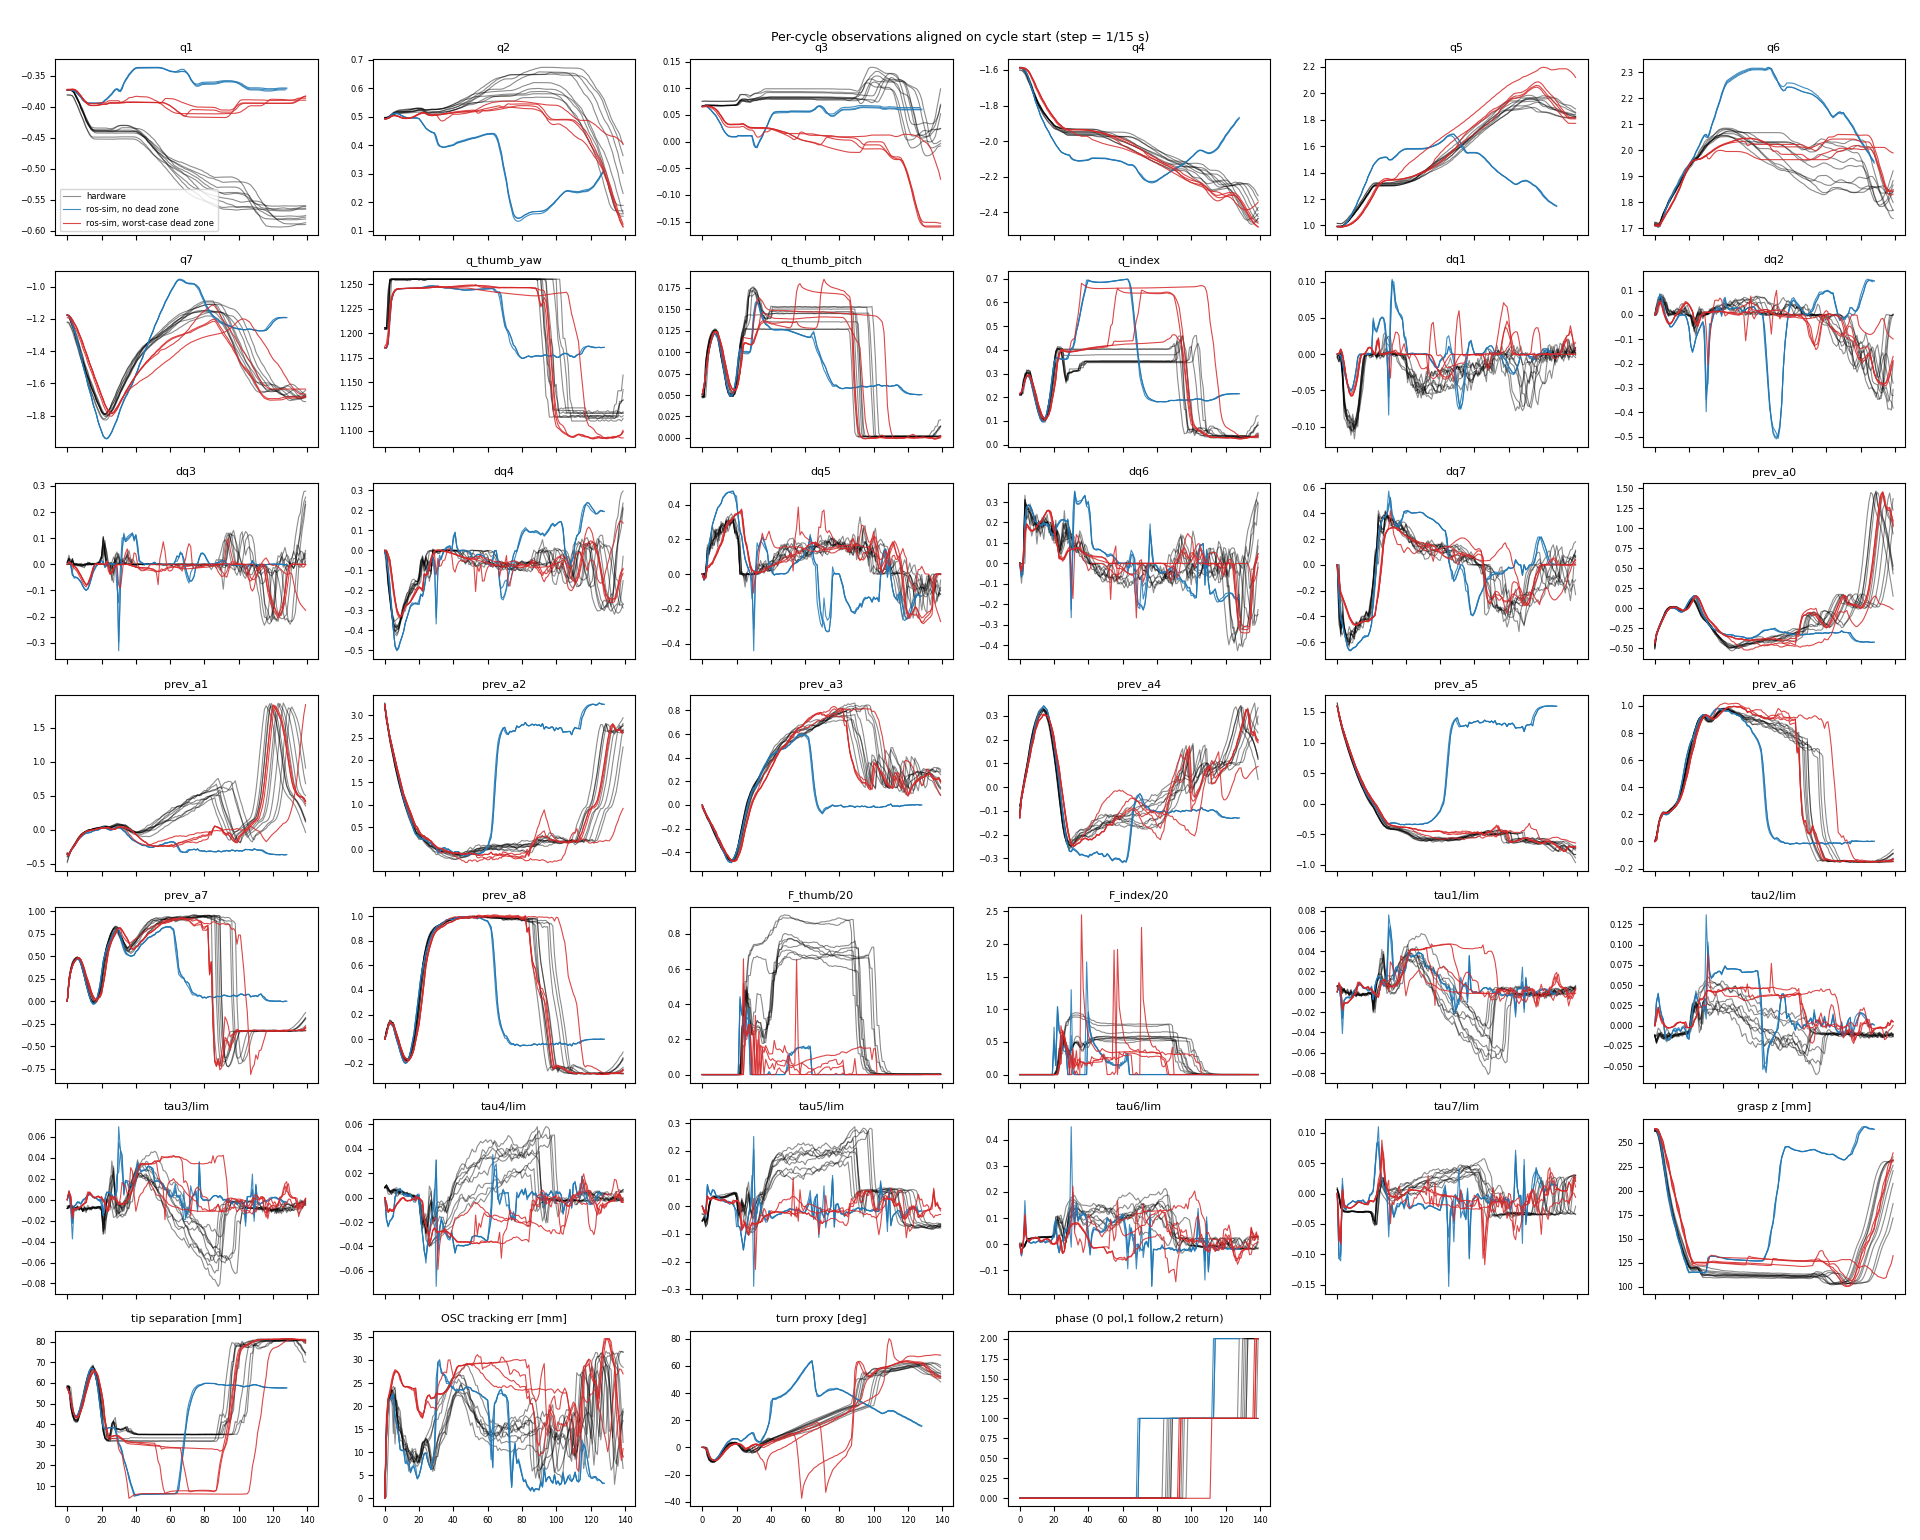
\includegraphics[width=\textwidth]{figures/controller/deadzone_proprio_overlay.png}%
    \caption[Observations per cycle on hardware and in ros-sim]{Observations of the proprio-friction student $S_1$ per cycle, aligned on the first policy step (one step is 1/15\,s). Black: nine hardware cycles of two runs. Blue: ros-sim without the dead zone. Red: ros-sim with the worst-case dead zone of 5\,N and 1\,N\,m. Panels show the student's proprioception (joint positions and velocities, previous action, pad forces, arm torques divided by the joint limit) and, in the last row, grasp height, fingertip separation, controller tracking error, the turn proxy, and the process phase.}%
    \label{fig:ctrl-dz-overlay}%
\end{figure}%

\paragraph{Interpretation.} The match of the policy length, the wrist joints, and the previous actions indicates that the worst-case dead zone reproduces how the physical arm follows the student's targets in free space. The return comparison shows that hardware and the dead-zone simulation are still turning back at the moment the gate's orientation bound is met, while the simulation without the dead zone has already finished turning. The mirrored offsets of j1 and j3 indicate that the redundant degree of freedom drifts in opposite directions in the two systems. The grasp gap is consistent with the contact argument of Section~\ref{sec:app-ctrl-dz-train}: the dead zone makes free-space motion sticky but leaves the arm compliant against contact forces.

\paragraph{Limitations.} The ros-sim side has seven cycles, and only one of them completed. At least one hardware run used friction compensation, and the ros-sim runs did not. The ros-sim arm carries the MuJoCo joint friction of 0.2\,N\,m per joint of the FR3 model it is built from, so the ``no dead zone'' condition is not frictionless. The run logs do not record whether the dead zone was on, so the assignment of the six ros-sim runs to the two conditions is inferred from the order in which they were run.

\section{Step-Aligned Comparison of the Return-Dead-Zone Student}\label{sec:app-ctrl-returndz}

\paragraph{Purpose and method.} The return-dead-zone student $S_2$ was trained with the dead zone in release and return only (Section~\ref{sec:app-ctrl-dz-train}). Its first hardware run was compared step by step with three ros-sim runs of the same checkpoint, one without the dead zone and two with the worst-case dead zone. All runs are aligned on the policy step and cut to the 99 steps of the hardware run, and the mean absolute difference per channel is computed in three windows. Whether friction compensation was active in the hardware run was not recorded.

\paragraph{Results.} On hardware, the first grip held from step 24 to about step 60 and was lost at step 63, after which the run was interrupted at step 100. The windows of the comparison are approach (steps 0--21), contact and hold (22--62), and after the slip (63--98). During the approach, the policy actions of all three ros-sim runs differ from hardware by at most 0.035 in normalized units per channel. Table~\ref{tab:ctrl-returndz} gives the grasp height and the vertical tracking error, and Figure~\ref{fig:ctrl-returndz} shows the grasp position.

\begin{table}[htb]%
    \centering%
    \caption[Grasp height and vertical error of the return-dead-zone student]{Grasp height and vertical controller error (target minus measured) of the return-dead-zone student $S_2$ per window, hardware against the ros-sim runs of the same checkpoint. Ranges over the steps of each window.}%
    \label{tab:ctrl-returndz}%
    \small
    \begin{tabular}{lcccc}
        \toprule
         & \multicolumn{2}{c}{Contact and hold (22--62)} & \multicolumn{2}{c}{After the slip (63--98)} \\
        Run & grasp $z$ [mm] & $z$ error [mm] & grasp $z$ [mm] & $z$ error [mm] \\
        \midrule
        hardware & 103.4--119.5 & $-10.3$ to 0.3 & 98.5--104.6 & $-3.9$ to 16.0 \\
        ros-sim, no dead zone & 114.0--133.0 & $-20.0$ to 0.5 & 125.8--127.9 & $-20.0$ \\
        ros-sim, worst case, run 1 & 125.0--127.6 & $-20.0$ to $-5.8$ & 123.7--125.1 & $-20.0$ \\
        ros-sim, worst case, run 2 & 124.6--132.2 & $-20.0$ to $-5.9$ & 126.6--128.8 & $-20.0$ \\
        \bottomrule
    \end{tabular}
\end{table}%

\begin{figure}[htb]%
    \centering%
    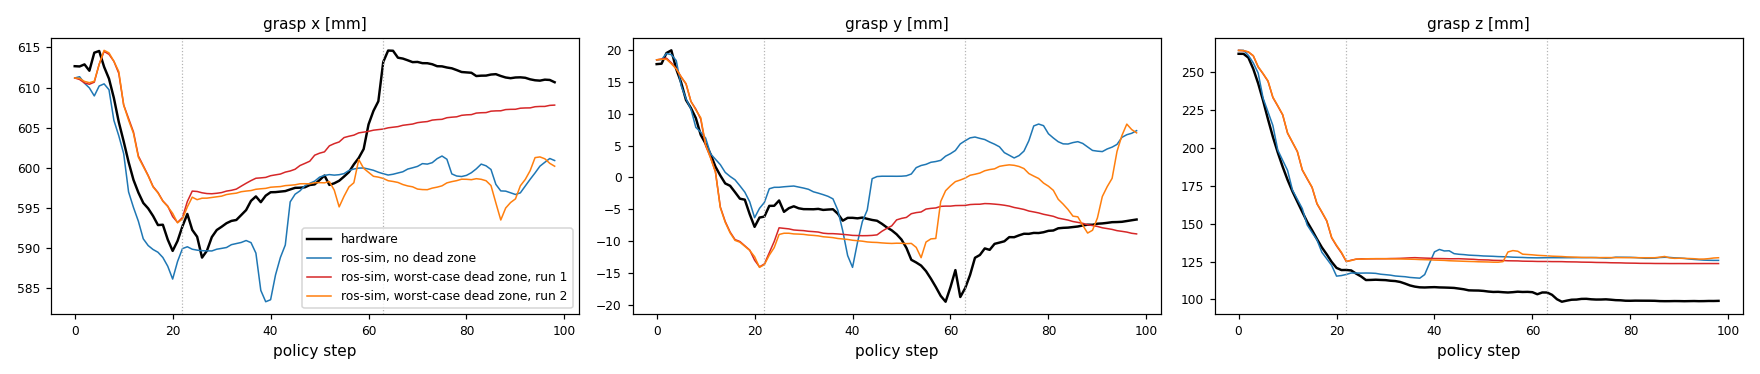
\includegraphics[width=\textwidth]{figures/controller/returndz_grasp_pos.png}%
    \caption[Grasp position of the return-dead-zone student]{Grasp position of the return-dead-zone student $S_2$ in the robot base frame on hardware (black) against ros-sim without the dead zone (blue) and with the worst-case dead zone (red and orange, two runs), aligned on the policy step. Dotted lines mark the first finger contact on hardware (step 22) and the slip (step 63).}%
    \label{fig:ctrl-returndz}%
\end{figure}%

After the slip step, the simulated hand is held at 123.7--128.8\,mm while its vertical error stays at the $-20$\,mm clip, so the controller pushes down at its limit and the hand does not descend. On hardware the hand descends to 98.5--119.5\,mm over the same steps. In the contact window, joints j4, j5, and j6 of the worst-case dead-zone runs differ from hardware by 0.007--0.042\,rad on average, against 0.125--0.207\,rad without the dead zone, while j7 differs by 0.066--0.072 against 0.097\,rad.

\paragraph{Interpretation.} The actions agree until contact, so the student receives equivalent observations in free space. From contact on, the two systems diverge because the simulated nut and the physical nut resist the hand differently. This is a contact gap that the arm controller does not address.

\paragraph{Limitations.} One hardware run and three ros-sim runs, all within the first 99 steps of a single cycle.

\section{Static Dead-Zone and Friction Probe}\label{sec:app-ctrl-probe}

\paragraph{Purpose and method.} The probe measures, at a fixed pose, how large a task-space wrench the physical arm holds without moving, in the units of the training dead zone. The characterization was designed in two parts, of which only part~A was built. The probe streams the policy goal along one base axis at a time, out to $+15$\,mm, back, rest, out to $-15$\,mm, back, and rest, at 6\,mm/s. Rotations use $\pm8\degree$ at $2\degree$/s. The analysis reads the 1\,kHz controller state and evaluates the spring wrench $-\mat{K}_p(\vec{x}_{\mathrm{measured}}-\vec{x}_{\mathrm{target}})$ per axis:
\begin{itemize}
  \item \emph{rest band}: where the arm settles at the start pose, approached once from each side. Half the difference of the two spring wrenches is the band, half their sum a bias, and the band divided by the stiffness is the stall distance.
  \item \emph{breakaway}: the spring wrench when the arm first follows the goal in a leg that starts from rest.
  \item \emph{creep}: the median spring wrench while the arm follows, reported after subtracting the expected damping share.
\end{itemize}
The rest band is the quantity a stalled return meets. The bias contains payload and gravity model errors. In the two sessions at pose o0, the hand load was set through libfranka on a zero-mass end-effector profile. The session at the return pose did not set it again.

\paragraph{Known-answer test in ros-sim.} With the worst-case dead zone, the probe recovers the thresholds as breakaway, 5.18--5.41\,N and 1.08--1.22\,N\,m over three runs at two speeds. Without the dead zone, the breakaway at the same pose is 0.05--0.15\,N and at most 0.03\,N\,m. The rest band, which only the later version of the probe records, reads 2.82--3.08\,N (5.0--5.5\,mm) and 1.17--1.30\,N\,m (2.4--2.7\degree) with the worst-case dead zone. Without the dead zone, at the return pose, it reads 0.28--1.18\,N and 0.46--0.64\,N\,m.

\paragraph{Results on hardware.} Of six hardware sessions, three ended before the first probe leg with an error. The other three completed. Table~\ref{tab:ctrl-probe} lists their rest bands next to the ros-sim known-answer runs.

\begin{table}[htb]%
    \centering%
    \caption[Rest band of the static probe]{Rest band of the static probe per base axis, in N or N\,m with the corresponding stall distance in mm or degrees in parentheses. Pose o0 places the grasp point at $(0.30,0.20,0.30)$\,m. The return pose is probed once with the arm in the reset posture and once in the posture in which a return had stalled. Friction compensation, where activated, is 0.3\,N\,m per joint.}%
    \label{tab:ctrl-probe}%
    \resizebox{\textwidth}{!}{%
    \begin{tabular}{lllcccccc}
        \toprule
        System & Pose & Condition & $x$ & $y$ & $z$ & $r_x$ & $r_y$ & $r_z$ \\
        \midrule
        hardware & o0 & no friction compensation & 1.72 (3.0) & 1.25 (2.2) & 1.94 (3.4) & 0.80 (1.6) & 0.82 (1.7) & 0.77 (1.6) \\
        hardware & o0 & friction compensation activated & 0.92 (1.6) & 1.12 (2.0) & 1.84 (3.3) & 0.86 (1.8) & 0.71 (1.4) & 0.52 (1.1) \\
        hardware & return, reset posture & friction compensation activated & 0.90 (1.6) & 0.82 (1.5) & 1.61 (2.8) & 1.14 (2.3) & 0.43 (0.9) & 0.37 (0.8) \\
        hardware & return, drifted posture & friction compensation activated & 1.10 (1.9) & 0.97 (1.7) & 2.11 (3.7) & 1.01 (2.1) & 0.47 (1.0) & 0.34 (0.7) \\
        \midrule
        ros-sim & o0 & worst-case dead zone & 2.88 (5.1) & 2.82 (5.0) & 3.08 (5.5) & 1.30 (2.7) & 1.17 (2.4) & 1.19 (2.4) \\
        ros-sim & return, reset posture & no dead zone & 1.18 (2.1) & 0.28 (0.5) & 0.46 (0.8) & 0.46 (0.9) & 0.55 (1.1) & 0.64 (1.3) \\
        \bottomrule
    \end{tabular}}
\end{table}%

At both poses the physical arm holds 0.8--2.1\,N and 0.34--1.14\,N\,m, which is 1.5--3.7\,mm and 0.7--2.3\degree. With friction compensation, the band at o0 shrinks on $x$ from 1.72 to 0.92\,N and on $r_z$ from 0.77 to 0.52\,N\,m, and changes by at most 0.13 on the other axes. The drifted posture raises the translational band by 0.15--0.50\,N over the reset posture. Every hardware run has a positive $z$ bias at rest, $+1.27$ to $+2.07$\,N. Without friction compensation, the creep wrench minus the damping share is 1.71--2.23\,N and 0.43--0.60\,N\,m, larger than the breakaway of the same session, 0.86--1.29\,N and 0.45--0.79\,N\,m.

\paragraph{Interpretation.} At these two poses, the rest band of the physical arm is smaller than the band that the worst-case dead zone produces in the same probe, 2.8--3.1\,N and 1.2--1.3\,N\,m. That the arm needs more spring wrench to keep moving than to start moving indicates a speed-dependent drag rather than stick-slip, and the breakaway values on hardware are therefore not a reliable friction estimate. Section~\ref{sec:app-ctrl-sweep} measures this drag directly. The positive $z$ bias is consistent with a payload model error but is not resolved by this test.

\paragraph{Limitations.} Two poses, one probe speed, and one session per condition. The payload fit that the same sessions record is ill-conditioned (condition number about 290) and is not used here.

\section{Lost Wrench against Speed}\label{sec:app-ctrl-sweep}

\paragraph{Purpose and method.} A dead zone and joint friction differ most in how the wrench they remove depends on speed. Once the arm moves in ros-sim, the dead zone removes the full threshold $d_i$ at any speed, whereas friction can grow with speed. The probe of Section~\ref{sec:app-ctrl-probe} was therefore repeated at four goal speeds per axis, 2, 6, 20, and 50\,mm/s and 1, 2, 6, and 15\degree/s, at pose o0 without setting the load. Every leg lasts at least 1.5\,s, so the faster levels use longer strokes, up to $\pm75$\,mm and $\pm22.5\degree$. For every moving sample of every leg, the analysis computes the lost wrench along the leg direction, the part of the spring wrench that does not go into the controller's damping,
\begin{equation}\label{eq:lost-wrench}
  \ell=-\mat{K}_p\,e-\mat{K}_d\,v,
\end{equation}
with $e$ the tracking error and $v$ the speed along the leg, both signed in the leg direction. The arm's inertia is ignored. Samples of both directions are folded together, binned by speed, and the bin medians, weighted with the square root of the bin count, are fitted with
\begin{equation}\label{eq:loss-curve}
  \ell(v)=F_c\tanh\!\left(\frac{v}{v_0}\right)+b\,v.
\end{equation}
$F_c$ is a Coulomb step smoothed over the speed $v_0$, and $b$ is a viscous coefficient. The training dead zone corresponds to $F_c=d_i$, $v_0\to0$, and $b=0$. A straight-line fit through the leg ends is not used, because it assumes that the arm reaches the goal speed within a leg, which the physical arm does not.

Three sessions completed: ros-sim without the dead zone, and hardware without and with friction compensation. The hardware session with friction compensation ran about half an hour after the one without, on a warmer arm. Two further ros-sim sessions ended early. The sweep was not run in ros-sim with a dead zone. For that case, the known-answer test of Section~\ref{sec:app-ctrl-probe} stands in: there the worst-case dead zone reads back as a breakaway of 5.18--5.41\,N and 1.08--1.22\,N\,m.

\paragraph{Results.} Table~\ref{tab:ctrl-sweep} lists the fitted terms, and Figure~\ref{fig:ctrl-sweep} shows the binned losses with the fits for the $x$ and $r_x$ axes. Without friction compensation, the physical arm loses 0.13\,N on $x$ at 0.15\,mm/s, 1.65\,N at 0.76\,mm/s, 2.82\,N at 1.3\,mm/s, 3.63\,N at 4.9\,mm/s, 5.06\,N at 17\,mm/s, and 6.97\,N at 44\,mm/s, with 6.32\,N on $y$ at 44\,mm/s. ros-sim loses 1.59\,N and 1.76\,N on $x$ and $y$ at 51\,mm/s. With friction compensation, the physical arm loses 4.93\,N on $x$ at 43\,mm/s and 3.92\,N on $y$ at 45\,mm/s.

\begin{table}[htb]%
    \centering%
    \caption[Fitted loss curve per axis]{Fit of \eqref{eq:loss-curve} to the lost wrench per axis at pose o0. $F_c$ in N or N\,m, $v_0$ in mm/s or deg/s, $b$ in N\,s/m or N\,m\,s/rad. The $z$ axis is left out: on hardware its fitted $v_0$ sits at the lower bound of the search grid, and its slowest bin already reads 2.8\,N, a static offset rather than friction (Section~\ref{sec:app-ctrl-probe}). The last row gives the training dead zone for comparison.}%
    \label{tab:ctrl-sweep}%
    \resizebox{\textwidth}{!}{%
    \begin{tabular}{llccccc}
        \toprule
        Condition & Term & $x$ & $y$ & $r_x$ & $r_y$ & $r_z$ \\
        \midrule
        hardware, no friction compensation & $F_c$ & 2.76 & 2.43 & 1.31 & 1.63 & 0.81 \\
         & $v_0$ & 0.96 & 1.17 & 0.60 & 0.89 & 0.73 \\
         & $b$ & 97.5 & 92.3 & 7.8 & 1.0 & 1.8 \\
        \midrule
        hardware, friction compensation activated & $F_c$ & 1.43 & 1.44 & 0.98 & 1.08 & 0.40 \\
         & $v_0$ & 0.96 & 1.34 & 0.73 & 0.96 & 0.68 \\
         & $b$ & 84.7 & 54.3 & 5.0 & 1.0 & 1.3 \\
        \midrule
        ros-sim, no dead zone & $F_c$ & 1.57 & 1.47 & 0.71 & 0.63 & 0.35 \\
         & $v_0$ & 1.43 & 1.53 & 0.68 & 0.68 & 0.89 \\
         & $b$ & 0.6 & 5.8 & 0.6 & 0.7 & 0.3 \\
        \midrule
        training, worst-case dead zone & $F_c$, $v_0$, $b$ & 5, 0, 0 & 5, 0, 0 & 1, 0, 0 & 1, 0, 0 & 1, 0, 0 \\
        \bottomrule
    \end{tabular}}
\end{table}%

\begin{figure}[htb]%
    \centering%
    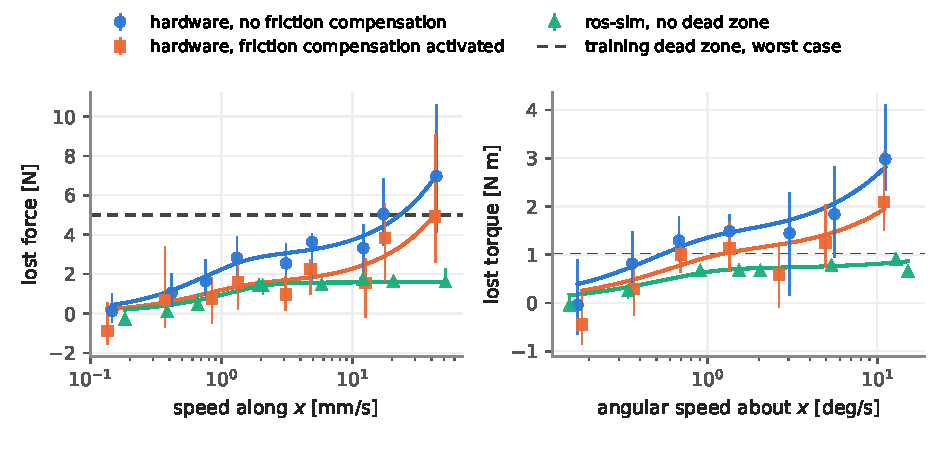
\includegraphics[width=\textwidth]{figures/controller/loss_curves.pdf}%
    \caption[Lost wrench against speed]{Lost wrench \eqref{eq:lost-wrench} against speed at pose o0, translation along $x$ (left) and rotation about $x$ (right), on hardware without and with friction compensation and in ros-sim without the dead zone. Markers are bin medians, bars the 25th to 75th percentile, lines the fits of \eqref{eq:loss-curve}. Dashed: the worst-case training dead zone, which removes its full threshold at any speed.}%
    \label{fig:ctrl-sweep}%
\end{figure}%

The raw signals of a single leg (no friction compensation, $x$, 2\,mm/s) show what the fit summarizes. On the outward leg the lag behind the goal grows from 0.2\,mm to 8.3\,mm over 6.6\,s and is still 7.9\,mm at the end of the 7.5\,s leg. Over the second half the arm moves at 1.46\,mm/s against the goal's 2.00\,mm/s, so it never reaches the goal speed. When the goal returns to the start pose and stops, the arm keeps approaching it for about 1.2\,s, from 2.6\,mm to 2.1\,mm short, and then rests.

The joint friction fit of Section~\ref{sec:app-ctrl-fit} does not account for the viscous part. Its per-joint viscous coefficients, though poorly identified, predict the task-space loss through the power balance $F_{\mathrm{pred}}=\sum_j b_j\dot{q}_j^2/v$, evaluated on the logged joint velocities of the 20 and 50\,mm/s legs. With the coefficients fitted on the day of the sweep, it predicts 0.09--0.13\,N at 16--18\,mm/s and 0.28--0.35\,N at 43--45\,mm/s, and with the largest coefficient of each joint over all seven days at most 0.82\,N. The fitted viscous term $b\,v$ of Table~\ref{tab:ctrl-sweep} is 2.4--4.1\,N at the same speeds.

\paragraph{Interpretation.} The physical arm does not lose a constant wrench once it moves. Its loss rises over the first millimeter per second to 2.4--2.8\,N and 1.3--1.6\,N\,m about $r_x$ and $r_y$, and keeps rising with speed at 92--98\,N\,s/m, about twice the controller's own translational damping of 47.5\,N\,s/m. Because the step is spread over $v_0\approx1$\,mm/s rather than being sharp, a small error is corrected slowly rather than held. The arm creeps, as the single leg shows, instead of sticking and slipping. ros-sim reproduces a smaller step, 1.5\,N, from the 0.2\,N\,m joint friction of its MuJoCo model, and no viscous term. The training dead zone is a sharp step without a viscous term. In translation, its worst case of 5\,N is larger than the hardware step of 1.4--2.8\,N, and in rotation its 1\,N\,m lies within the hardware range of 0.4--1.6\,N\,m. At policy speeds the viscous term dominates: at 44\,mm/s the physical arm loses about 7\,N on $x$ without friction compensation, against 1.6\,N in ros-sim. The joint viscous coefficients of the same day account for at most a seventh of the fitted viscous term, and the largest coefficients over all days for at most 0.27 of it, so its source remains open. With friction compensation, $F_c$ halves on $x$ and $y$ and $b$ drops from 92--98 to 54--85\,N\,s/m. Because that session ran on a warmer arm, this is an upper bound on the effect of friction compensation.

\paragraph{Limitations.} One pose, one session per condition, and the warm-up confound between the two hardware sessions. Inertia is neglected in \eqref{eq:lost-wrench}, which affects the bins near the turnarounds. The $z$ axis is distorted by a static offset and is not evaluated.

\section{Why the Return Stalls}\label{sec:app-ctrl-stall}

\paragraph{Purpose and method.} On hardware, the Cartesian return to the reset pose stops short of it, whereas the joint-space re-home lands within a few millimeters. The torques at such a stall were decomposed for two hardware runs. In the second, the return gate of 3\,mm and $2\degree$ never passed, so the return ran for its full 16.9\,s. The logged state is averaged from 4\,s into the return onward, and the position spring and the rotation spring are mapped separately to joint torques through $\mat{J}^{\mathrm{T}}$.

\paragraph{Results.} In the second run, the arm settled 3.7\,s into the return at 16--17\,mm and $7\degree$ with all joints below 0.006\,rad/s, and then crept to 14.5\,mm and $5.9\degree$. Averaged over the rest, the error is 15.8\,mm and $6.4\degree$, the spring force $(8.33,-3.18,0.82)$\,N, and the spring torque $(-0.60,1.86,2.46)$\,N\,m. Table~\ref{tab:ctrl-stall} gives the joint torques.

\begin{table}[htb]%
    \centering%
    \caption[Joint torques at a return stall]{Joint torques at the return stall of the second run, from the position spring and the rotation spring separately, their sum, and the commanded torque recorded at rest, in N\,m.}%
    \label{tab:ctrl-stall}%
    \small
    \begin{tabular}{lccccccc}
        \toprule
         & j1 & j2 & j3 & j4 & j5 & j6 & j7 \\
        \midrule
        position spring & $-2.10$ & $-0.93$ & $-1.72$ & 3.64 & 0.93 & 2.22 & $-0.13$ \\
        rotation spring & 2.46 & 0.99 & 1.63 & $-2.02$ & $-2.11$ & $-2.11$ & 0.18 \\
        sum (task torque) & 0.36 & 0.06 & $-0.10$ & 1.62 & $-1.18$ & 0.10 & 0.05 \\
        recorded command & 0.85 & 0.00 & 0.16 & 1.45 & $-1.18$ & $-0.08$ & 0.15 \\
        \bottomrule
    \end{tabular}
\end{table}%

The two springs oppose each other on j1--j6. What remains is 1.6\,N\,m on j4 and $-1.2$\,N\,m on j5, and neither joint moves. The first run shows the same pattern: a 13.7\,mm position error with 7.7\,N and a rotation spring of about 3.5\,N\,m reach 3.8\,N\,m at single joints, but the net torque is at most 1.5\,N\,m. The exact nullspace projector contributes at most 0.04\,N\,m there, so the posture term does not move the arm back either.

\paragraph{Interpretation.} The grasp point lies 185\,mm from the flange, close to $\sqrt{28/565}=0.22$\,m. For a rotation of the hand about a point near the wrist, the position spring and the rotation spring therefore nearly cancel, and the effective stiffness about the flange is $28-565\cdot0.185^2\approx8.7$\,N\,m/rad, a third of the rotational gain. A small friction torque on j4 and j5 holds a large combined error in this direction. Because j4 and j5 do not move under the residual torque, their static friction at this posture is at least 1.5 and 1.2\,N\,m. The probe of Section~\ref{sec:app-ctrl-probe} excites one task axis at a time and never this coupled direction, which explains why it reads a small band while the return stalls at about 9\,N. The law has no integral term, in training as on hardware, so any error held by friction persists.

\paragraph{Limitations.} Two stalls at one return pose. The static friction bounds are lower bounds inferred from the absence of motion.

\section{Transition Clip}\label{sec:app-ctrl-tclip}

\paragraph{Purpose and implementation.} The policy clip of 0.02\,m and 0.097\,rad bounds the target step against the measured pose in every 1\,kHz cycle, and so it also bounds the spring wrench to $565\cdot0.02=11.3$\,N and $28\cdot0.097=2.7$\,N\,m per axis. During the scripted transitions of the cycle, waypoint following and the return to reset, a goal may now widen the clip and the fault limits up to the ceilings of Table~\ref{tab:ctrl-fixed}. The hardware runs below use a transition clip of 0.05\,m and 0.25\,rad, the value of the training configuration.

\paragraph{Clip speed limit.} With critical damping, a target clipped to $\delta$ ahead of the arm drives it at a steady speed of at most $\mat{K}_p\delta/\mat{K}_d=\delta\sqrt{\mat{K}_p}/2$. This gives 0.24\,m/s and 0.26\,rad/s for the policy clip and 0.59\,m/s and 0.66\,rad/s for the transition clip. These are derived values for a pure translation or rotation of a lossless arm. Section~\ref{sec:app-ctrl-repeat} measures the speed while the policy clip is active: 178\,mm/s in ros-sim and 95--128\,mm/s on the physical arm, whose loss grows with speed (Section~\ref{sec:app-ctrl-sweep}).

\paragraph{Method and data.} Six hardware runs of the proprio-friction student $S_1$ used the transition clip. Runs 1--3 recorded the 1\,kHz controller state, which is aligned with the rollout log to evaluate each transition phase. Runs 4--6 have the 15\,Hz rollout log only. Runs 1 and 2 did not re-home between cycles, and runs 3--6 did. The return gate was 15\,mm and $10\degree$ in run 1 and 20\,mm and $10\degree$ afterward.

\paragraph{Results.} Table~\ref{tab:ctrl-tclip} gives the transition phases of runs 2 and 3, and Figure~\ref{fig:ctrl-tclip} shows run 2. In earlier runs with the policy clip in the transitions, orientation had stopped at 16--20\degree\ during the return. With the transition clip, every return of runs 1--5 that passed the gate did so within 2.0--2.7\,s, and no run hit a tracking fault. With re-homing, 12 of 12 cycles completed in runs 3--5. Without re-homing, the position error at the end of the return grew from cycle to cycle, 13.0, 15.6, and 17.3\,mm in run 2, while the arm posture drifted within every cycle, about $-0.2$\,rad on j1 and $+0.2$\,rad on j3, and the drift carried into the next cycle. With re-homing it stayed at 12.5--13.5\,mm. In run 1, cycle 2 did not pass the 15\,mm gate and stopped at 15.2\,mm and $6.7\degree$ after 16.9\,s. Run 6 ended in cycle 1 when the grip collapsed during the turn.

\begin{table}[htb]%
    \centering%
    \caption[Transition phases with the transition clip]{Transition phases with the transition clip (0.05\,m, 0.25\,rad, fault limits 0.1\,m and 0.5\,rad) on hardware, runs 2 and 3, three cycles each. Ranges over cycles. Errors are against the clipped target.}%
    \label{tab:ctrl-tclip}%
    \small
    \begin{tabular}{lcc}
        \toprule
        Quantity & Waypoint following & Return to reset \\
        \midrule
        duration & 2.87\,s & 2.27--2.67\,s \\
        fraction of the phase with orientation clipped & 0.26--0.30 & 0.53--0.59 \\
        fraction of the phase with position clipped & 0 & 0 \\
        peak position error & 0.041--0.057\,m & 0.056--0.067\,m \\
        peak orientation error & 0.406--0.441\,rad & 0.358--0.364\,rad \\
        \bottomrule
    \end{tabular}
\end{table}%

\begin{figure}[htb]%
    \centering%
    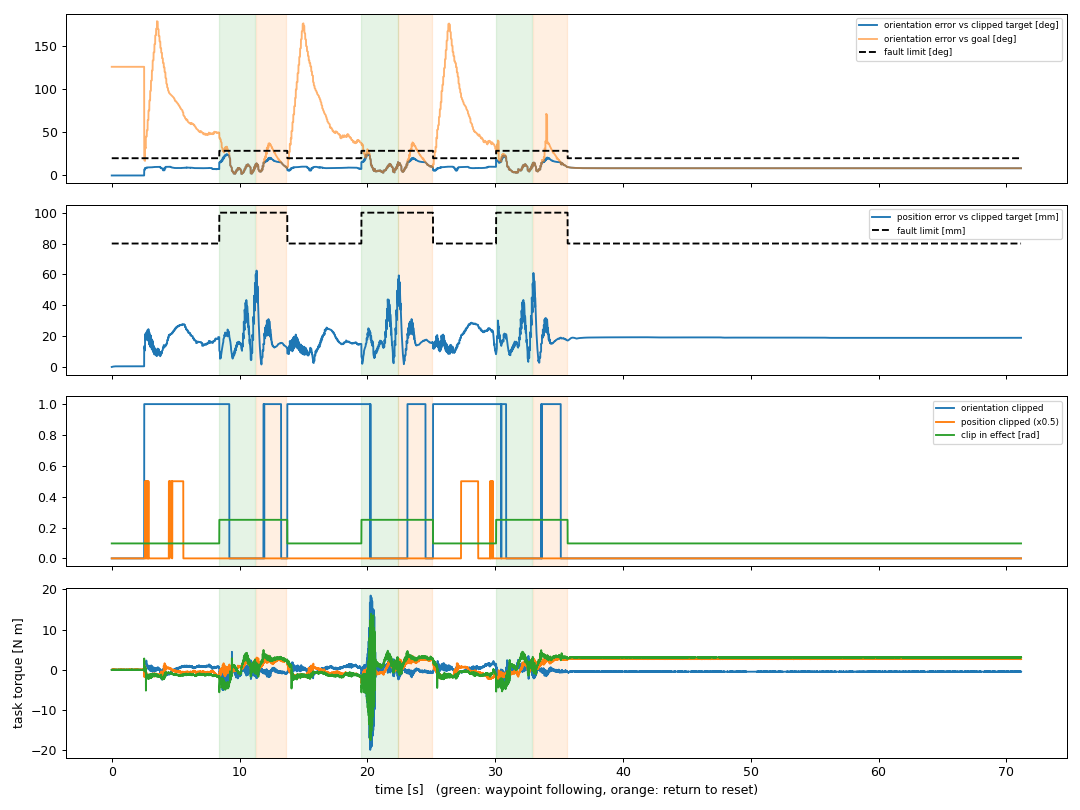
\includegraphics[width=0.9\textwidth]{figures/controller/transition_clip_hw_run2.png}%
    \caption[Transition clip on hardware]{Transition clip on hardware, run 2 (three cycles without re-homing), from the 1\,kHz controller state. From top to bottom: orientation error against the clipped target and against the goal with the fault limit, position error with the fault limit, clip flags and the orientation clip in effect, and the task torque. Green bands mark waypoint following, orange bands the return to reset.}%
    \label{fig:ctrl-tclip}%
\end{figure}%

\paragraph{Interpretation.} The wider clip raises the spring wrench that a transition can apply, and this fixed the orientation stall of the return. It does not fix the position residual, which is the coupled stall of Section~\ref{sec:app-ctrl-stall}. The gate fired while the arm was still closing at 3--5\,mm/s and 10--16\degree/s, so the residuals at the gate are not resting points. The growth without re-homing follows the accumulated drift of j1 and j3, which the nullspace spring of stiffness 10 does not undo against friction.

\paragraph{Limitations.} The peak orientation error of 0.441\,rad leaves a margin of 0.06\,rad to the 0.5\,rad fault limit. Only runs 1--3 have 1\,kHz data, and no per-phase summary is available for run 1. The ros-sim recordings of the same comparison are not evaluated here.

\section{Target Accuracy and Repeatability}\label{sec:app-ctrl-repeat}

\paragraph{Purpose and method.} A repeatability test streams the policy goal between two grasp positions in the base frame, A at $(0.30,0.20,0.30)$\,m and B at $(0.30,0.40,0.30)$\,m, at several orientations, and approaches every target from both sides. The goal moves at up to 0.5\,m/s, faster than the policy clip lets the arm follow, so the arm runs into the clip on the way. At each arrival, the goal stops on the target and the rest error is the mean over the last 0.5\,s of the hold. From the arrivals of one target, the test computes the \emph{accuracy} (distance of the mean rest position from the target, ISO~9283 style), the \emph{repeatability} per approach side, the \emph{hysteresis} (distance between the mean rest positions of the two sides, from friction or a dead zone), and the \emph{bias} (their mean, from a load or model error). It also counts the arrivals inside 5\,mm and 5\degree. In the earlier runs every hold lasted a fixed 2\,s. In the later runs, a hold lasts until the arm has moved less than 0.2\,mm and 0.1\degree\ over 0.5\,s, at least 2\,s and at most 10\,s, and every arrival records whether it settled.

\paragraph{ros-sim.} Five ros-sim runs were made, all without the dead zone. Three completed, one stopped near a singularity, and one was rejected because a joint ended 0.22\,rad from the start posture. Table~\ref{tab:ctrl-repeat} lists the completed runs.

\begin{table}[htb]%
    \centering%
    \caption[Accuracy and repeatability in ros-sim]{Accuracy and repeatability of the controller in ros-sim without the dead zone, two positions $\times$ four orientations, each approached from both sides. All arrivals ended inside 5\,mm and $5\degree$.}%
    \label{tab:ctrl-repeat}%
    \small
    \begin{tabular}{lccccc}
        \toprule
        Run & Arrivals & Accuracy (mean) & Worst repeatability & Hysteresis (mean) & Peak speed \\
        \midrule
        1 & 32 & 1.07\,mm & 2.22\,mm / 2.60\degree & 2.15\,mm & 0.257\,m/s \\
        2 & 16 & 1.05\,mm & 2.16\,mm / 2.53\degree & 2.19\,mm & 0.332\,m/s \\
        3 & 16 & 1.27\,mm & 1.32\,mm / 0.35\degree & 1.31\,mm & 0.228\,m/s \\
        \bottomrule
    \end{tabular}
\end{table}%

\paragraph{Hardware runs.} Three early hardware attempts stopped before their first arrival. In one, the controller rejected a goto step of 3.03\,rad, one was interrupted, and one was rejected because the start posture was 0.71\,rad from the checked one. Of five later runs, four completed and one was rejected at the start, because the forward kinematics of the measured joints disagreed with the robot's end-effector pose. The two runs used for accuracy were made about ten minutes apart, one without and one with friction compensation. Each has 40 arrivals, two positions $\times$ orientations o0 (flange down) and o1 ($30\degree$ yaw) $\times$ two sides $\times$ five repeats, and every arrival settled. Two earlier runs, again one without and one with friction compensation, have 80 arrivals at four orientations with a fixed 2\,s hold. They are used below only for arrival speed, not for accuracy. Table~\ref{tab:ctrl-repeat-hw} gives the results of the two settled runs. The error 1\,s after the goal stopped and the median speed of the grasp point while the position clip was active were computed from the 50\,Hz pose samples.

\begin{table}[htb]%
    \centering%
    \caption[Accuracy and repeatability of the physical arm]{Accuracy and repeatability of the physical arm, 40 settled arrivals per run at A and B, orientations o0 and o1, both sides, five repeats. Per-target values are listed as A/o0, A/o1, B/o0, B/o1. Friction compensation, where activated, is 0.3\,N\,m per joint.}%
    \label{tab:ctrl-repeat-hw}%
    \resizebox{\textwidth}{!}{%
    \begin{tabular}{lcc}
        \toprule
        Quantity & No friction compensation & Friction compensation activated \\
        \midrule
        hold after the goal stopped & 2.00--2.49\,s & 2.00--2.02\,s \\
        accuracy (mean over targets) & 8.54\,mm & 6.42\,mm \\
        arrivals inside 5\,mm and $5\degree$ & 0 of 40 & 5 of 40, all at A/o0 \\
        hysteresis (mean) & 6.07\,mm & 3.78\,mm \\
        hysteresis per target & 10.4, 1.5, 0.3, 12.1\,mm & 5.1, 2.0, 0.2, 7.8\,mm \\
        repeatability per approach side & 2.2--3.3\,mm & 1.7--2.8\,mm \\
        $z$ bias per target & $-3.5$, $-2.7$, $-4.2$, $-5.6$\,mm & $-2.8$, $-1.2$, $-5.6$, $-5.4$\,mm \\
        load implied by the $z$ bias (mean, range) & 0.23\,kg (0.16--0.32) & 0.22\,kg (0.07--0.32) \\
        \midrule
        error 1\,s after the goal stopped (median) & 18.2\,mm & 6.9\,mm \\
        speed while the position clip is active (median) & 95\,mm/s & 128\,mm/s \\
        \bottomrule
    \end{tabular}}
\end{table}%

Within a target and side, the rest error changes from the first to the fifth repeat by $-0.5$ to $+2.6$\,mm without friction compensation and by $-0.6$ to $+2.1$\,mm with it, and grows in six of eight cases in both runs. Over the same five repeats, the rest posture drifts by $-0.24$ to $-0.42$\,rad on j1 and $+0.20$ to $+0.37$\,rad on j3. The earlier runs give the same order between the two settings. The median error 1\,s after the goal stopped is 19.9\,mm without and 7.6\,mm with friction compensation, and the median speed with the position clip active is 86 and 126\,mm/s. In ros-sim (run 1 of Table~\ref{tab:ctrl-repeat}) it is 178\,mm/s.

\paragraph{Interpretation.} The physical arm is precise but not accurate: per approach side, it returns within 1.7--3.3\,mm, but it rests 6--9\,mm from the target on average. Part of the repeatability spread is the drift of the redundant joints j1 and j3 over the repeats, the same drift as in Section~\ref{sec:app-ctrl-tclip}. The hysteresis averages 4--6\,mm but ranges from 0.2 to 12\,mm between targets, large at A/o0 and B/o1 and small at B/o0 and A/o1, in both runs. Joint friction maps to task space through the posture-dependent Jacobian, so its band depends on the target. A per-axis task-space band, such as the dead zone, cannot represent this. Friction compensation reduces the mean hysteresis by 38\,\% and the mean accuracy error by 25\,\%, and it makes the arm arrive faster (6.9 instead of 18.2\,mm after 1\,s). It does not change the downward $z$ bias of 1--6\,mm, which corresponds to about 0.2\,kg of unmodeled load. That bias is therefore a payload or gravity-model error, not friction.

The clip-limited speed follows from the loss curve of Section~\ref{sec:app-ctrl-sweep}. With the clip at $\delta=0.02$\,m, the spring wrench is at most $\mat{K}_p\delta=11.3$\,N, and in steady motion it balances $\mat{K}_d v+F_c+b\,v$. With the $y$ fits of Table~\ref{tab:ctrl-sweep}, this gives 63\,mm/s without friction compensation, 97\,mm/s with it, and 184\,mm/s in ros-sim. ros-sim moves at that speed (178\,mm/s), and the physical arm moves about 30\,mm/s faster than predicted but in the same order. The loss curve was measured at a single pose and on single axes, whereas the transits combine both. Between runs with the same setting, made 40 to 60 minutes apart, the clip-limited speed changes by 10\,\% (86 and 95\,mm/s) and 2\,\% (126 and 128\,mm/s), and the error after 1\,s by 1.7 and 0.7\,mm. Switching friction compensation on changes the same quantities by a factor of 1.3 to 2.6. Any effect of warm-up is therefore smaller than the effect of friction compensation. It was not measured separately.

\paragraph{Limitations.} Two positions, two orientations, and one settled run per setting. The two earlier runs have unsettled holds and are not used for accuracy. Arrivals from the same side follow the same transit, so the repeatability per side does not include the spread of different approach paths.

\section{Joint Friction Fitted from Rollouts}\label{sec:app-ctrl-fit}

\paragraph{Purpose and method.} Ordinary policy rollouts already contain a friction signal. The joint torque sensor of the \ac{FR3} sits between gearbox and link, so the difference between the desired torque $\tau_{J,d}$ and the measured link-side torque minus gravity is torque lost in the gearbox. This holds also in contact, because external forces act on the link side. The lost torque is computed from the logged desired and measured joint torques of the hardware rollouts (low-pass filtered with 0.02\,s) and fitted per joint and day, on samples with $|\dot{q}_j|>0.01$\,rad/s, with
\begin{equation}\label{eq:friction-fit}
  \tau_{J,d,j}-\left(\tau_{J,j}-g_j\right)=\tau_{c,j}\operatorname{sign}(\dot{q}_j)+b_j\dot{q}_j+o_j,
\end{equation}
with Coulomb friction $\tau_{c,j}$, viscous coefficient $b_j$, and offset $o_j$. Friction compensation, when activated, is part of $\tau_{J,d}$, so the fit measures the total friction either way.

\paragraph{Results.} Table~\ref{tab:ctrl-fit} lists the Coulomb terms of 56 runs on seven days over two weeks.

\begin{table}[htb]%
    \centering%
    \caption[Joint Coulomb friction fitted from rollouts]{Coulomb friction $\tau_c$ per joint of the physical \ac{FR3}, in N\,m, fitted from hardware rollouts per day with \eqref{eq:friction-fit}. Days are numbered in chronological order over two weeks. The last row gives the correlation between the lost torque and $\operatorname{sign}(\dot{q})$ over the days. For j1 it is undefined on two days.}%
    \label{tab:ctrl-fit}%
    \resizebox{\textwidth}{!}{%
    \begin{tabular}{lcccccccc}
        \toprule
        Day & Runs & j1 & j2 & j3 & j4 & j5 & j6 & j7 \\
        \midrule
        1 & 6 & 0.32 & 0.86 & 0.40 & 0.50 & 0.58 & 0.30 & 0.26 \\
        2 & 6 & 0.31 & 0.88 & 0.29 & 0.56 & 0.59 & 0.33 & 0.26 \\
        3 & 11 & 0.35 & 0.87 & 0.42 & 0.55 & 0.58 & 0.29 & 0.24 \\
        4 & 5 & 0.54 & 0.93 & 0.48 & 0.64 & 0.43 & 0.37 & 0.24 \\
        5 & 17 & 0.58 & 0.97 & 0.45 & 0.60 & 0.54 & 0.23 & 0.24 \\
        6 & 8 & 0.60 & 0.82 & 0.37 & 0.64 & 0.60 & 0.32 & 0.26 \\
        7 & 3 & 0.61 & 0.89 & 0.33 & 0.65 & 0.60 & 0.32 & 0.21 \\
        \midrule
        correlation & & 0.70--0.87 & 0.93--0.97 & 0.58--0.88 & 0.54--0.96 & 0.90--0.98 & 0.55--0.93 & 0.79--0.95 \\
        \bottomrule
    \end{tabular}}
\end{table}%

The Coulomb friction is 0.21--0.97\,N\,m depending on the joint. It is largest on j2 (0.82--0.97\,N\,m), and on j1 it roughly doubled from 0.31--0.35\,N\,m on days 1--3 to 0.54--0.61\,N\,m from day 4 on. The other joints vary by at most 0.19\,N\,m over the seven days. The viscous coefficients scatter between $-0.01$ and 4.86\,N\,m\,s/rad. They are not used as a friction model, only for the rough comparison in Section~\ref{sec:app-ctrl-sweep}.

\paragraph{Interpretation.} The physical joints have 0.2--1\,N\,m of Coulomb friction. The training recipes with joint friction draw 0.16--0.4\,N\,m per joint (0.2\,N\,m scaled by $U(0.8,2.0)$). Joints j2, j4, and j5 exceed that range on every day, and j6 and j7 lie inside it. The uniform friction compensation of 0.3\,N\,m lies below the fitted friction on j1--j5 but above it on j7 (0.21--0.26\,N\,m) and on j6 on two days (0.23 and 0.29\,N\,m). This disagrees with the rationale that 0.3\,N\,m stays below every measured moving loss, which rested on two earlier runs (Section~\ref{sec:app-ctrl-additions}). A per-joint compensation from Table~\ref{tab:ctrl-fit} would remove this inconsistency, but it has not been tried.

\paragraph{Limitations.} The rollouts are logged at 15\,Hz, the rotor inertia is ignored during accelerations, and the joints stay below about 1\,rad/s, so the viscous term is not identifiable. The two hardware runs of Section~\ref{sec:app-ctrl-rollout}, the second stall run of Section~\ref{sec:app-ctrl-stall}, and the transition-clip runs of Section~\ref{sec:app-ctrl-tclip} are not part of the fit, although they contain the desired torque.

\section{Summary}\label{sec:app-ctrl-summary}

Training models the imperfection of the arm as a sharp, memoryless, speed-independent step in task space, the dead zone of up to 5\,N and 1\,N\,m. The physical \ac{FR3} under the same impedance law behaves differently in four measured respects. First, it loses a Coulomb step smoothed over about 1\,mm/s, 2.4--2.8\,N and 0.8--1.6\,N\,m without friction compensation, plus a viscous term of 92--98\,N\,s/m, about twice the controller's damping (Table~\ref{tab:ctrl-sweep}). Second, the low-speed part is smaller than the worst-case dead zone in translation and similar in rotation: the static probe reads a rest band of 0.8--2.1\,N and 0.3--1.1\,N\,m (Table~\ref{tab:ctrl-probe}), and the joint Coulomb friction fitted from 56 rollouts over seven days is 0.2--1\,N\,m (Table~\ref{tab:ctrl-fit}). Third, at policy speeds the viscous part dominates: at 44\,mm/s the arm loses about 7\,N against 1.6\,N in ros-sim, and with the position clip active it moves at 95--128\,mm/s against 178\,mm/s in ros-sim. Fourth, the loss depends on the posture. The hysteresis between approach sides ranges from 0.2 to 12\,mm between targets (Table~\ref{tab:ctrl-repeat-hw}), and in the coupled direction of a rotation about the wrist the same friction holds a return about 15\,mm and $6\degree$ from its target (Section~\ref{sec:app-ctrl-stall}). Because the arm creeps rather than sticks, the error it ends with depends on how long it is given.

A task-space dead zone gets the order of magnitude of the rest band right, which is why the worst-case dead zone in ros-sim reproduces the free-space motion and the return of the physical arm (Section~\ref{sec:app-ctrl-rollout}). It misses the speed dependence, the posture dependence, and the creep. In contact it leaves the hand free to move inside the band, where the physical arm resists (Sections~\ref{sec:app-ctrl-dz-train} and~\ref{sec:app-ctrl-returndz}). The deployment controller therefore adds three measures: joint friction compensation on hardware, which reduces the hysteresis by 38\,\% and the accuracy error by 25\,\% (Section~\ref{sec:app-ctrl-repeat}); the training dead zone as an option in ros-sim; and the wider transition clip, which fixed the orientation stall of the return (Section~\ref{sec:app-ctrl-tclip}). The physical arm remains offset 6--9\,mm from its targets, including a downward $z$ bias of 1--6\,mm that friction compensation does not change and that points to a payload or gravity-model error. The remaining gap between ros-sim and hardware lies mostly in contact and grasping, which the arm controller does not address.
